\documentclass[dvipdfmx,line_length=48zw,column_gap=2zw,number_of_lines=60,baselineskip=12pt]{jlreq}
\jlreqsetup{itemization_beforeafter_space=0pt}
\makeatletter
\RenewBlockHeading{section}{1}{font={\jlreq@keepbaselineskip{\normalsize\sffamily\gtfamily}},indent=0pt,lines=1}
\RenewBlockHeading{subsection}{2}{font={\jlreq@keepbaselineskip{\normalsize\sffamily\gtfamily}},indent=0pt,lines=1}
\RenewBlockHeading{subsubsection}{3}{font={\jlreq@keepbaselineskip{\normalsize\sffamily\gtfamily}},indent=0pt,lines=1}
\makeatother
\pagestyle{empty}
% ↑この上の部分は変更しない！
% （LuaTeXを使う場合は \documentclass[dvipdfmx,... の dvipdfmx, を消す）
%%%%%%%%%%%%%%%%%%%%%%%%%%%

%%↓必要なパッケージを追加してください．
\usepackage{mathtools,amssymb}
\usepackage{latexsym}
\usepackage{newtxtext,newtxmath}
\usepackage[utf8]{inputenc} 	%波ダッシュ（〜）を表記できるようにする
\newcommand{\red}[1]{\textcolor{red}{#1}}
\newcommand{\cut}[1]{\textcolor{red}{\sout{\textcolor{black}{#1}}}}
%%%%%%%%%%%%%%%%%%%%%%%%%%%

\begin{document}
\twocolumn[
    {\Large
            \begin{center}
                %%↓タイトルを入力してください
                % 卒業論文のタイトルを書く
長期に活動する男性アイドルグループの歌詞分析
                %%%%%%%%%%%%%%%%%%%%%%%%%%%
            \end{center}
        }
    \vspace{12pt}
    \begin{flushright}
        福知山公立大学情報学部　32145037　金梨沙 \\
        指導教員　橋田光代
    \end{flushright}
    \vspace{1\Cvs}
]

%% ここから本文を書く
% !TEX root = _yoko.tex
\def\sectionmargin{\vspace{7pt}}

% ==========================================
% プロジェクトω予稿（1P）の本文
% ==========================================

\red{chatGPTによる自動要約はこんな。びっくりするほど表面的（＝外面だけをなぞっていて、研究した本人ならではの
    勢いある文章では全然ない。これが「かっこいい・すごい・良い」とは思わないように。いわゆる「意識高い系」）}

\section{概要}
本研究では、合成音声に朗読表現を付加するシステムを検討する。朗読は単なる情報伝達を超え、音の表現により文章の意味や話者の感情を伝える役割を持つ。しかし、既存の合成音声は自然な発話表現に乏しく、朗読のような豊かな表現を再現することが難しい。本研究では、合成音声ソフト「VOICEPEAK」をベースに、発話表現を制御可能なシステムをPythonで構築し、実験的評価を行った。

\sectionmargin
\section{研究背景}
文章だけでは意味が曖昧になりやすい。例えば、「頭が赤い魚を食べる猫」という文は、音声表現の違いにより異なる解釈を生む（図\ref{fig:redcat1}）。朗読では音の区切りや抑揚が適切に付与され、情報が正確に伝わる。特に、感情や意図を伴う朗読表現では、話し手の意図や文脈の流れが強調されるため、リスナーが文章の意図を適切に理解しやすくなる。

また、現代の合成音声技術では、イントネーションやリズムの制御は可能であるものの、感情を込めた朗読のような自然な表現には限界がある。本研究では、音声の強弱やテンポの調整を可能にすることで、より多様な発話表現を実現する。

\sectionmargin\section{提案手法}

\subsection{発話表現の制御機能}
朗読の発話表現を分析し、音の強弱、速度、抑揚を調整できる機能を実装した。具体的には、VOICEPEAKで生成した音声に対し、音響特徴を変化させるアルゴリズムを開発し、ユーザが発話表現を選択・設定できるシステムを構築した。本システムでは、音声のピッチや速度を制御するだけでなく、句読点や文脈に応じた適切なポーズを加えることで、より自然な表現を可能にする。

\subsection{多様な発話スタイルの生成}
音声データに対して事前に学習させた朗読表現の特徴を適用し、異なる発話スタイルを持つ複数の音声を生成できるよう設計した。これにより、ユーザーが目的に応じた朗読表現を柔軟に選択できるようになった。加えて、音声の韻律情報を考慮した調整機能を導入し、従来よりも流暢で滑らかな発話を可能にした。ユーザの入力に応じてリアルタイムにフィードバックを提供する機能も実装し、直感的な調整を容易にした。


\sectionmargin
\section{実験と評価}


\sectionmargin
\subsection{聴取実験の実施}
本システムを用いて異なる発話表現の合成音声を作成し、被験者20名に聴取実験を実施した。評価では、各発話パターンごとに自然さ、感情表現の明瞭さ、理解のしやすさを5段階評価で測定した。その結果、提案手法により抑揚や速度が異なる音声の識別が容易になり、より自然で感情豊かな朗読表現が再現可能であることが確認された。


\sectionmargin
\subsection{比較実験}
さらに、比較実験として、従来の合成音声と本システムで生成した音声の聞き取りテストを実施した。結果として、提案手法を用いた音声は「より自然に聞こえる」「抑揚が明確で聴きやすい」との評価が多く得られた。また、発話速度やポーズの調整による理解度の向上も確認され、特に長文の朗読において顕著な効果が見られた。

被験者のフィードバックを基にさらなる改良を検討し、発話の個人差や異なる感情表現のバリエーションを取り入れることで、より高品質な合成音声を実現できる可能性が示唆された。

\sectionmargin
\section{結論}
本研究では、朗読表現を取り入れた合成音声システムを提案し、実験を通じてその有効性を示した。具体的には、抑揚や発話速度、ポーズの制御を組み合わせることで、リスナーにとってより自然な音声を生成できることを確認した。

今後の課題としては、より細かい発話制御機能の追加や、多様な話者の表現に対応するシステムの拡張が挙げられる。また、ディープラーニングを活用した自動朗読表現の最適化や、リアルタイムでの発話調整機能の開発も視野に入れている。特に、話者の個性を反映したパーソナライズ可能な朗読合成技術の確立が求められる。




\sectionmargin
\begin{figure}[tb]
    \centering
    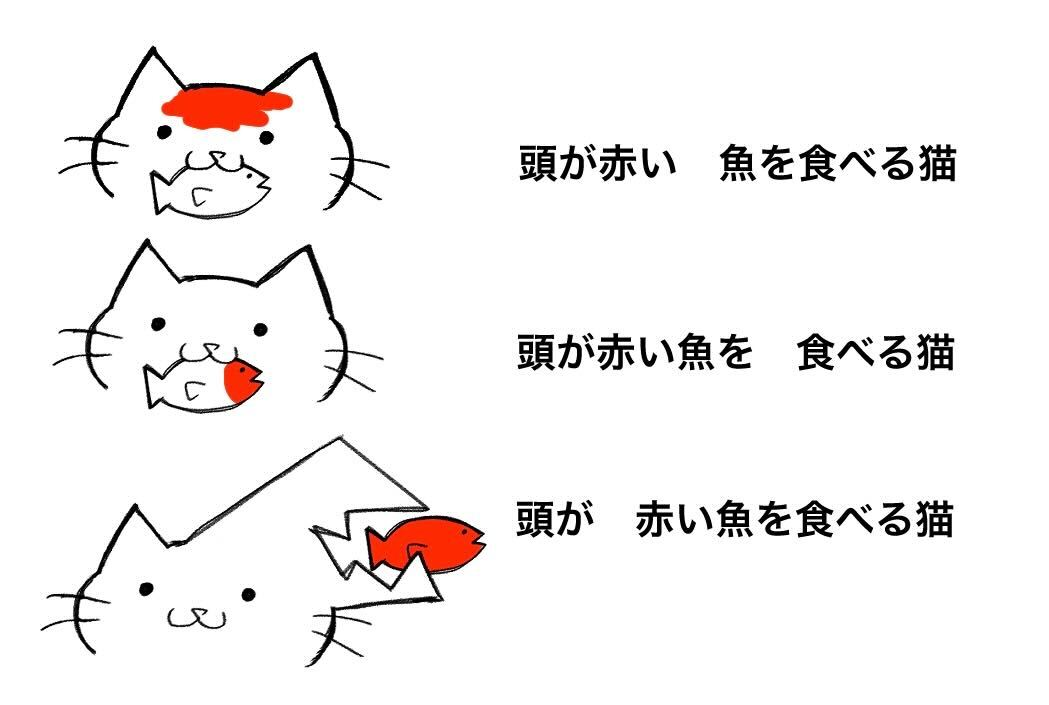
\includegraphics[width=0.8\linewidth]{fig/osakana.jpg}
    \caption{音で伝える「頭が赤い魚を食べる猫」\\（文献\cite{akaineko}を参考に筆者作成）}
    \label{fig:redcat1}
\end{figure}


% 参考文献
\vspace{10pt}
\scriptsize
\bibliographystyle{muselabunsrt} % bstファイルの名前
\bibliography{koyama2025} % .bibファイルの名前（Zoteroからエクスポートして作る）

\end{document}
